\documentclass{article}
\usepackage[a4paper]{geometry}
\usepackage{tikz}

\def\spiral#1{
	\pgfmathparse{int(#1)}
	\ifnum\pgfmathresult > 0
	\draw [black!20] (0, 0) rectangle (1, 1);
	\begin{scope}[shift={(1,1)}, rotate=-90, scale=1/1.6180339887]
		\spiral{#1-1}
	\end{scope}
	\draw [black!80,very thick] (0, 0) arc (180:90:1);
	\fi
}

\begin{document}
	\begin{center}
		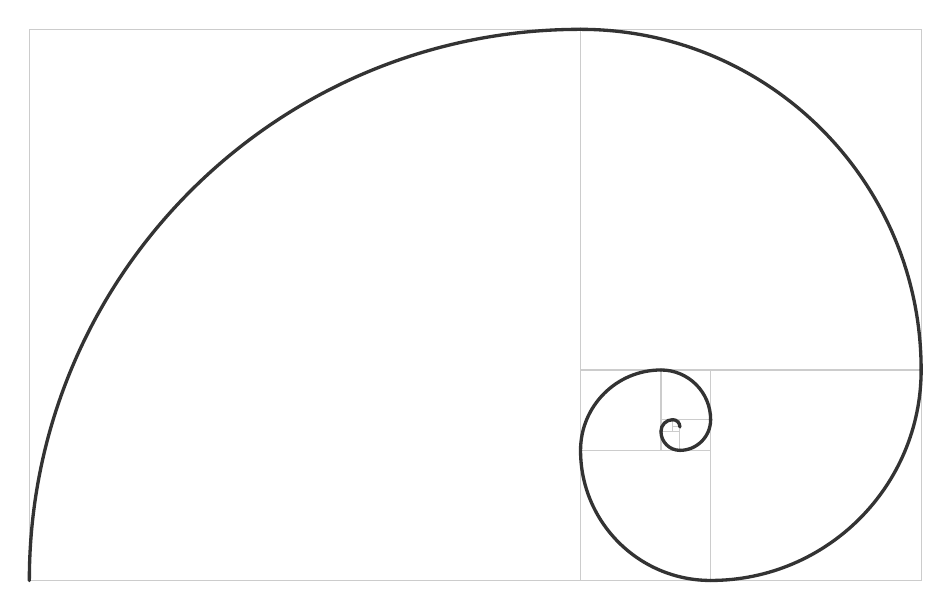
\begin{tikzpicture}[line cap=round]
			\begin{scope}[scale=7]
				\spiral{10}
			\end{scope}
		\end{tikzpicture}
	\end{center}
	
	
	\begin{Huge}
		\[
		F_n = \frac{1}{\sqrt{5}}\left [ \left ( \frac{1 + \sqrt{5}}{2}  \right )^n -  \left ( \frac{1 - \sqrt{5}}{2}  \right )^n \right ]  
		 \]
	\end{Huge}
\end{document}